\documentclass[a4paper,12pt]{jsarticle}
\bibliographystyle{junsrt}
\usepackage{ascmac}
\usepackage{empheq}
\usepackage{amsmath,amssymb}
\usepackage{bm}
\usepackage[dvipdfmx]{graphicx,color}
\usepackage[top=30truemm,bottom=30truemm,left=30truemm,right=30truemm]{geometry}
\usepackage[format=hang,margin=75pt,font=small]{caption}
\usepackage{here}
\usepackage{comment}
\title{レーザー歪み計を用いた基線長安定化制御の提案}
\author{三代浩世希}
\begin{document}
\setcounter{tocdepth}{3}
\maketitle
\abstract{}
\tableofcontents

\section{基線長安定化のための能動防振}
\subsection{能動防振に求めるもの}
能動防振システムの性能は以下の3つで評価できる
\begin{enumerate}
\item \textbf{外乱抑制性能} ステージへの地面振動の流入をどれぐら抑えられるか 
\item \textbf{即応性能} RMSをどれぐらい小さく抑えられるか
\item \textbf{目標値追従性能} 干渉計からの制御信号にどれぐらい追従させられるか
\end{enumerate}

(制御の目的は上記の3つを改善すること。その説明をする。)

(外乱抑制と目標追従を両立させるために2自由度制御をつかう。)

(2自由度制御は、LIGOでも使われているが、sensor correction として呼ばれている。)


\subsection{従来の能動防振}

Pre-Isolatorの目的はステージを慣性系に対して静止させることである。したがってFeedBackで用いるセンサーには慣性センサーを用いなければならない。しかし図\ref{img:img_seismo_vs_lvdt}が示すように、一般的に慣性センサーは低周波で地面振動よりもノイズが大きいため、ループゲインを低周波で大きくすることができず、ステージのDC位置を慣性系に対して静止させることができない。

一方で、共振器長制御のためには、ステージの位置制御をしなければならない。そのため低周波ではローカルな変位センサーをつかって、地面の揺れに追従するようにしている。このように慣性センサーと変位センサーをあわせたセンサーのことを super sensor と呼ぶ\cite{hua2005low}。低周波でノイズが大きくなる慣性センサーには high-pass フィルターを、変位センサーには同じカットオフ周波数のlow-pass フィルターをかけており、これらフィルターは相補フィルターと呼ばれており、以下のような関係式で結ばれる。
\begin{eqnarray}\label{eq:eq01}
  L(\omega) + H(\omega) = 1
\end{eqnarray}  
ここで、$L(\omega),\,L(\omega)$はそれぞれlow-passフィルターとhigh-passフィルターである。このような super sensor を用いて、高周波では慣性系に、低周波では地面に対してFeedBack制御をおこなっている。。

\begin{figure}[H]
  \begin{center}
    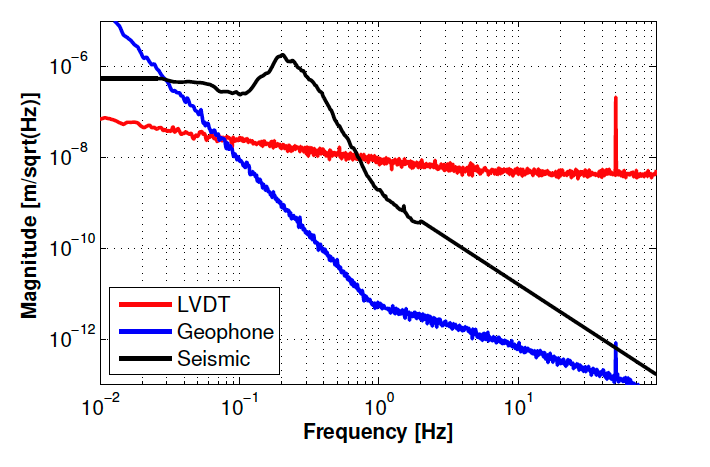
\includegraphics[width=10.0cm]{./img_seismo_vs_lvdt.png}
  \end{center}
  \caption{地面振動とセンサーノイズの比較。黒線は地面振動。赤線はLVDTのセンサーノイズ。青線はGeophoneのセンサーノイズ。およそ0.1 Hz以上ではGeophoneが、それ以下ではLVDTのセンサーノイズが小さい。参考文献\cite{sekiguchiD2016}のFig5.6から転載。}
  \label{img:img_seismo_vs_lvdt}
\end{figure}


\begin{figure}[H]
  \begin{center}
    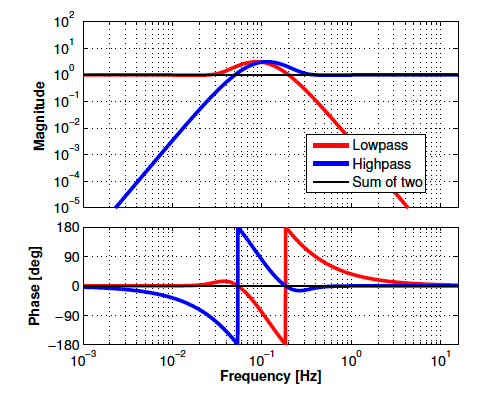
\includegraphics[width=10.0cm]{./img_pi_blending.png}
  \end{center}
  \caption{Blendingフィルター。0.1Hzにカットオフ周波数をもつ相補フィルター。図\ref{img:img_seismo_vs_lvdt}によれば、0.1Hz以下の低周波ではLVDTの信号を、それ以上ではGeophoneの信号をあわせたいので、ローパスをLVDTに、ハイパスをGeophoneにかける。参考文献\cite{sekiguchiD2016}のFig5.8から転載。}
  \label{img:img_pi_blending}
\end{figure}

変位センサーを使うということは、ステージが地面と一緒に動くことを意味している。これは比較的小さいスケールの腕共振器であれば、低周波地面振動は同相な地面振動雑音として除去されるので問題とならない。しかしkmスケールの腕共振器では、とくにRMSの大きな脈動の帯域では、逆相成分である基線長伸縮は同相成分とくらべて1/4程度にしか低減できない[]。このような問題に対してLIGOではsensor correction と呼ばれるfeed forward 制御を用いた試みをおこなっている\cite{hua2005low}\cite{matichard2015seismic}。


\begin{figure}[H]
  \begin{center}
    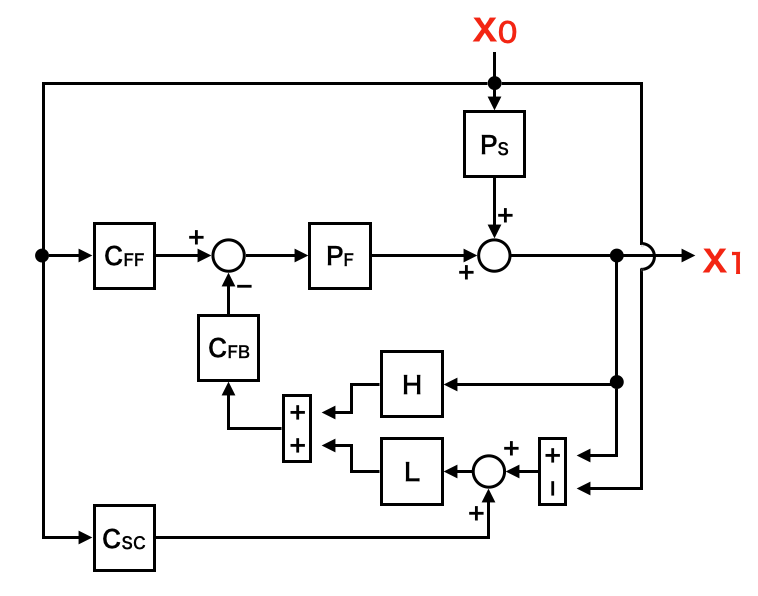
\includegraphics[width=10.0cm]{./img_2dof_pi.png}
  \end{center}
  \caption{Preisolatorで用いている能動防振のブロック図。ここで、$P_{\mathrm{s}}$は地面振動の変位$x_0$からステージの変位$x_1$への伝達関数である。$C_{\mathrm{fb}},\,C_{\mathrm{ff}},\,C_{\mathrm{sc}}$はそれぞれ feedback、feedforward、sensor correctionの制御フィルターである。さらに$H,\,L$はsuper sensor のための相補フィルターであり、それぞれ慣性センaサーのためのハイパスフィルターと変位センサーのためのローパスフィルターである。また$N_{ff},\,N_{sc},\,N_{H},\,N_{L}$はそれぞれのセンサーのノイズとなっている。そして$G$はループゲインをあらわしており$G=C_{\mathrm{fb}}P_{\mathrm{f}}$という関係であり、このときの$P_{\mathrm{f}}$はステージのアクチュエータからステージの変位への伝達関数である。}\label{img:img_2dof_pi}
\end{figure}


Sensor correction について述べる。LIGOの能動防振のブロック図を図\ref{img:img_2dof_pi}に示す。この図においてステージの変位$x_1$を地面振動$x_0$で表すと式(\ref{eq:eq04})の通りである。
\begin{eqnarray} \label{eq:eq04}
  x_1 &=& \frac{1}{1+G}\Biggl[(P_{\mathrm{s}}+P_{\mathrm{f}}C_{\mathrm{ff}})x_0\Biggl]
  + \frac{G}{1+G}\Biggl[L(1+C_{\mathrm{sc}})x_0\Biggl]
\end{eqnarray}
ここで低周波の外乱抑制を高めるために式(\ref{eq:eq04})のゲイン$G$を十分に大きくすると式(\ref{eq:eq06}),(\ref{eq:eq07})になる。式(\ref{eq:eq07})によれば、feed back のみの場合、ステージの変位$x_1$はローパスフィルター$L$(図\ref{img:img_pi_fb_sc_ff}の緑色の破線)に沿って地面振動$x_0$を流入させる(図\ref{img:img_pi_fb_sc_ff}の橙色の実線)。しかしsensor correction を加えて$C_{\mathrm{sc}}=-1$となるようにフィルターを作れば地面振動からの寄与を減らすことができる(図\ref{img:img_pi_fb_sc_ff}の茶色の実線)。
\begin{eqnarray}\label{eq:eq06}
  \lim_{G \to \infty} x_{1} &=& L(1+C_{\mathrm{sc}})x_0 \\
  &=&
  \begin{cases}\label{eq:eq07}
    \; Lx_{0} & \text{($C_{\mathrm{sc}}=0$)}\\
    \; 0 & \text{($C_{\mathrm{sc}}=-1$)} 
  \end{cases}  
\end{eqnarray}

実際のところ、sensor correction で用いる witness sensor には慣性センサーを使うので、supuer sensor と同様に、high-pass フィルターをつかってノイズの流入を抑えなければならない(図\ref{img:img_pi_fb_sc_ff}の青色の破線)。比較的低周波まで測定できる広帯域地震計であっても数$10\,\mathrm{mHz}$であるため、数分以上の位置制御は望めない。さらに、慣性センサーは低周波ではtilt coupling と呼ばれる傾斜成分が並進成分にカップルする性質があるため、むやみに低周波のゲインを大きくすることができない。近年、傾斜計を加えて傾斜成分を補償する試み\cite{biscansD2018}がなされているが、上述したように、地震計のノイズレベルで低周波の位置制御は制限されることに変わりはない。


ちなみにsensor correction とは別に、高周波帯域のステージの要求値を満たすために、もう一つのfeed forward を用意している。式(\ref{eq:eq08}),(\ref{eq:eq09})にゲインを小さくした場合のステージの変位$x_1$を示す。式(\ref{eq:eq08})によれば、feed back のみの場合は、ステージの変位$x_0$はステージの地面振動応答$P_{\mathrm{s}}$に沿って地面振動を流入させる(図\ref{img:img_pi_fb_sc_ff}の橙色の実線が示す$0.5\,\mathrm{Hz}$以上の高周波部分)。このとき、sensor correction と同様に、$C_{\mathrm{ff}}=\frac{P_{\mathrm{s}}}{P_{\mathrm{f}}}$となるようにフィルター(図\ref{img:img_pi_fb_sc_ff}の紫色の破線)をつくれば、地面振動からの寄与を減らすことができる。
\begin{eqnarray}\label{eq:eq08}
  \lim_{G \to 0} x_{1} &=& P_{\mathrm{s}}x_0 + P_{\mathrm{f}}C_{\mathrm{ff}}x_0 \\
  &=& 
  \begin{cases}\label{eq:eq09}
    \; P_{\mathrm{s}}x_{0} & \text{($C_{\mathrm{ff}}=0$)}\\
    \; 0 & \text{($C_{\mathrm{ff}}=\frac{P_{\mathrm{s}}}{P_{\mathrm{f}}}$)} 
  \end{cases}  
\end{eqnarray}

( この節をまとめる )


\begin{figure}[H]
  \begin{center}
    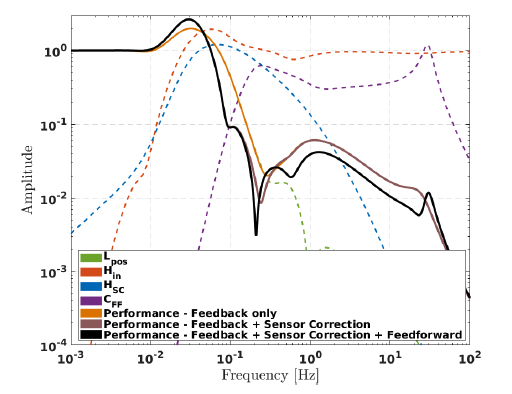
\includegraphics[width=11.0cm]{./img_pi_fb_sc_ff.png}
  \end{center}
  \caption{参考文献\cite{biscansD2018}のFig3.13から転載。}
  \label{img:img_pi_fb_sc_ff}
\end{figure}






\subsection{レーザー歪み計をつかった能動防振}
従来の方法では、ITMとETMはそれぞれのローカルな地面振動に対してロックしているため、基線長伸縮に地面振動の影響が現れてしまう。これはそれぞれの防振装置が、低周波に感度持たない慣性センサーで sensor correction を行うことに起因する。基線長制御においては基線長伸縮を補償すれば良い。

幸いKAGRAでは$x_0-y_0$を直接測ることができるレーザー歪み計\cite{araya2017design}があるため、これをsensor correction のセンサーとして利用する。レーザー歪み計は基線長伸縮に対して感度をもち、慣性センサーとくらべて、広いダイナミックレンジと広帯域という利点をもつ図(\ref{img:img_seismo_vs_gif})。

\begin{figure}[H]
  \begin{center}
    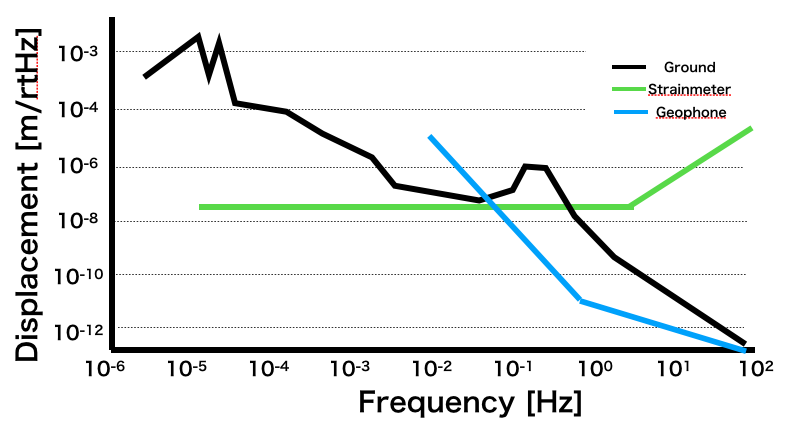
\includegraphics[width=10.0cm]{./img_seismo_vs_gif.png}
  \end{center}
  \caption{}\label{img:img_seismo_vs_gif}
\end{figure}



\begin{eqnarray}
  x_1 &=& \frac{1}{1+G}\Biggl[(P_{\mathrm{s}}+P_{\mathrm{f}}C_{\mathrm{ff}})x_0\Biggl]
  + \frac{G}{1+G}\Biggl[L(1+C_{\mathrm{sc}})x_0 - LC_{\mathrm{sc}}y_0\Biggl]
\end{eqnarray}
\begin{eqnarray}\label{eq:eq10}
  \lim_{G \to \infty} x_{1} &=& L\Biggl[x_0+C_{\mathrm{sc}}x_0-C_{\mathrm{sc}}y_0\Biggl] \\
  &=&  
  \begin{cases}\label{eq:eq11}
    \; Lx_{0} & \text{($C_{\mathrm{sc}}=0$)}\\
    \; Ly_{0} & \text{($C_{\mathrm{sc}}=-1$)} 
  \end{cases}  
\end{eqnarray}


\begin{figure}[H]
  \begin{center}
    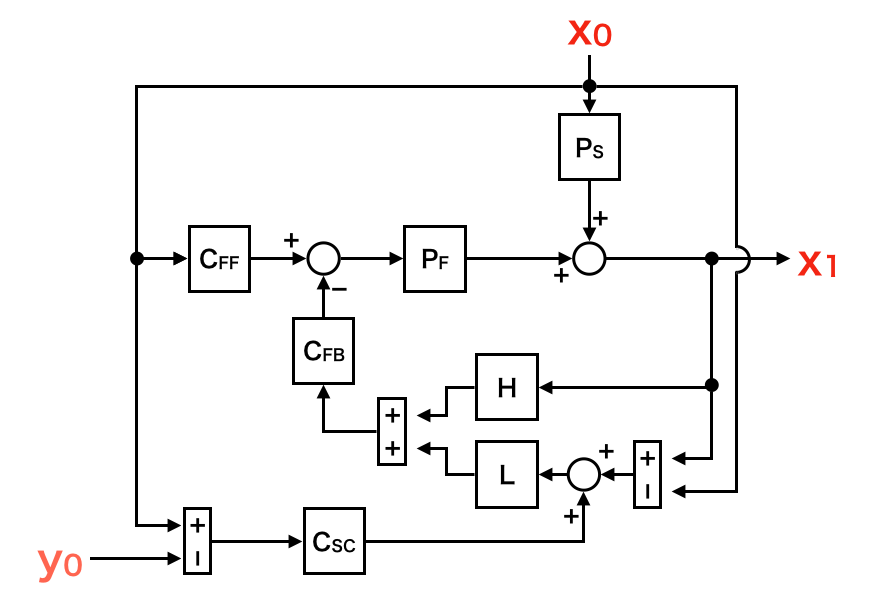
\includegraphics[width=10.0cm]{./img_pi_etmx.png}
  \end{center}
  \caption{}\label{img:img_pi_etmx}
\end{figure}






\appendix
\section{2自由度制御}

\begin{figure}[H]
  \begin{center}
    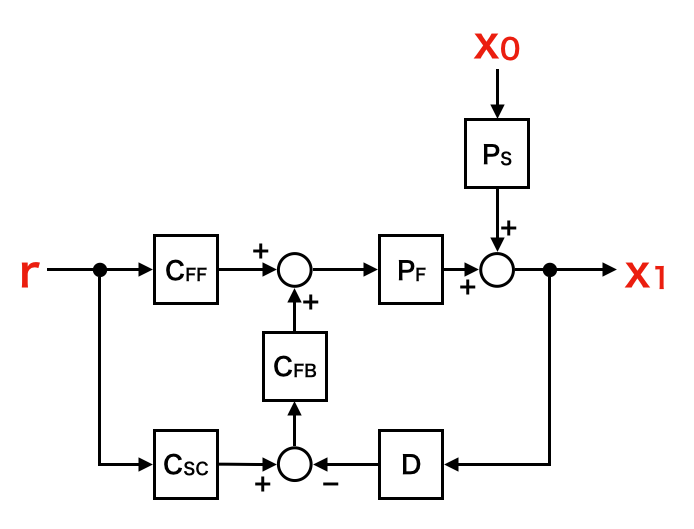
\includegraphics[width=10.0cm]{./img_2dof.png}
  \end{center}
  \caption{}\label{img:img_2dof}
\end{figure}

能動防振でつかわれている2自由度制御を説明するよりも先に、2自由度制御のひな形を用いて、2自由度制御の利点である、外乱抑制性能と目標追従性能の両方を向上できることを示しておかなければならない。まずステージの変位$x_1$を目標値$r$と外乱$x_0$で表すと式(\ref{eq:eqA01})のとおりになる。
\begin{eqnarray} \label{eq:eqA01}
  x_1 &=& \frac{1}{1+G}\Biggl[P_{\mathrm{s}}x_0 + P_{\mathrm{f}}C_{\mathrm{ff}}r\Biggl] + \frac{G}{1+G}\Biggl[\frac{C_{\mathrm{sc}}}{D}\Biggl]r
\end{eqnarray}
もし$C_{\mathrm{ff}}=1$かつ$C_{\mathrm{sc}}=0$であれば一般的なFeedBack制御になるが、2自由度制御では式(\ref{eq:eqA01})の第2項が加わるおかげで外乱抑制と目的値追従を両方とも良くすることができる。それはつまり外乱抑制をよくするためにGを大きくとると、
\begin{eqnarray} \label{eq:eqA02}
  \lim_{G \to \infty} x_1 = \frac{C_{SC}}{D}r
\end{eqnarray}
となり、適当な$C_{\mathrm{sc}}$を選べば、$x_{1}=r$となって、制御後の値$x_{1}$を目標値$r$に一致させることができるためである。

\section{式置き場}

\begin{eqnarray}
  d_1 &=& \frac{1}{1+G}P_{S}d_0 \\
  &+& \frac{G}{1+G}\Biggl[L(1-C_{SC})-\frac{C_{FF}+C_{GIF}}{C_{FB}}\Biggl]d_0 \nonumber \\
  &-& \frac{G}{1+G}\Biggl[HN_{H} + LN_{SC} + LN_{L} + \frac{C_{FF}}{C_{FB}}N_{FF} + \frac{C_{GIF}}{C_{FB}}N_{GIF} \Biggl] \nonumber
\end{eqnarray}

\begin{eqnarray}
  \lim_{G \to \infty} \langle|d_1|^2\rangle =
  \biggl\langle\biggl|[L(1-C_{SC})-\frac{C_{FF}+C_{GIF}}{C_{FB}}]d_0\biggl|^2\biggl\rangle + \langle|N_{\mathrm{all}}|^2 \rangle \\
N_{\mathrm{all}} \equiv HN_{H} + LN_{SC} + LN_{L} + \frac{C_{FF}}{C_{FB}}N_{FF} + \frac{C_{GIF}}{C_{FB}}N_{GIF} \nonumber
\end{eqnarray}
%
%


\bibliography{./reference}

\end{document}
